\documentclass[../main.tex]{subfiles}
\graphicspath{{\subfix{../Figures/}}}
\begin{document}
    \begin{frame}{Is this result as powerful as the one for graphs?} 
    	
		\begin{block}{Mixing in irregular hypergraphs}
			$I_t(k) - \pi(S_j(\bold{p}_{t})) \leq \sqrt{\frac{k}{d(v_0)}} e^{-\frac{t\hat{\phi}^2}{4}}$
		\end{block}
	
		$\frac{k}{d(v_0)}$ can be as large as $\Omega(2^n)$, which means that even if the mixing time is large $\Omega(n)$, we can only have the guarantee that the output conductance is a constant.    
	\end{frame}	

	\begin{frame}{Conductance is $O(1)$, but mixing is $O(n)$}
		\begin{lemma}
			There exists a multigraph s.t. the conductance is $\frac{1}{2}$ but the mixing time is $O(n)$.
		\end{lemma}
		Here is an example: \\ 
		\begin{center}
		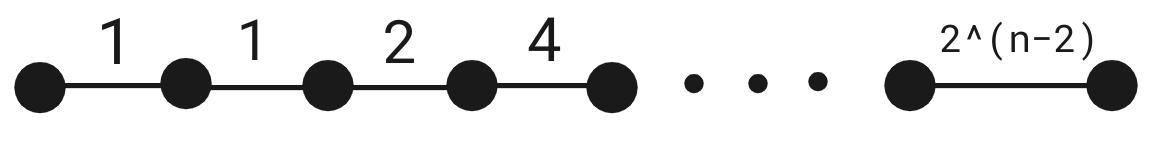
\includegraphics[width=0.5\textwidth]{Figures/path_graph}
		\end{center}
		\begin{itemize}
			\item Nodes $[1,n]$ in a straight path.
			\item Edge $(i,i+1)$ has weight $w(i,i+1) = \sum_{j=0}^{i} w(i,i+1)$ so that weight doubles at every $i$.
			\item Total graph volume: $2^{n-1}$.
			\item Conductance is $\frac{1}{2}$.
			\item Mixing time is $O(n)$ for a large fraction of nodes.
		\end{itemize}
	\end{frame}

	\begin{frame}{An argument for not having this issue in hypergraphs}
		Recall that the actual mixing theorem found with our analysis for the discrete diffusion process is
		\begin{block}{Improved mixing theorem for irregular hypergraphs}
			$I_t(k) - \pi(S_j(\bold{p}_t)) \leq \sqrt{\frac{k}{d(v_0)}}e^{-\frac{\hat{\phi}t}{
			4}}$
		\end{block}
		This means that when the volume of the hypergraph is exponential, then the probability of picking as starting node a vertex with non-exponential degree is very low.
	\end{frame}
\end{document}